\mySection{Principper}
\begin{multicols}{2}
  \begin{tList}{RIR - I morgen er der også en dag}

  \item Lad være med at gå helt til grænsen hver gang. Du bliver ikke
    stærkere af det, men du bliver trættere.
    Specifikt for den enkelte øvelse, altså hver sæt i
    styrketræning skal du ikke give max gas.

    Forskning indikerer, at det helt klart er
    muligt at blive stærkere, også selvom man ikke presser sig selv
    til grænsen hvert sæt. Det er især tilfældet for folk, der ikke
    har trænet den specifikke øvelse tidligere.
    \emph{$\rightarrow$ Eksempel: Du kan max tage 10 armbøjninger, så tag 8.}

  \item Generelt for hele sessionen. Det giver mening at klatre
    oftere med kortere sessioner i stedet for færre, som er længere.
    Lad være med at køre dig selv helt i smadder hver gang du
    klatrer. Du skal klatre igen senere på ugen.
    Hvis du kører en maratonsesh er du sikkert alligevel for træt
    til at få noget ud af det den sidste times tid.
    Så høj kvalitet som muligt hver session. Klatring er en teknisk sport.

  \end{tList}

  \begin{tList}{Progressive overload - stille og roligt mere og mere}
  \item Kroppen tilpasser sig det, det du udsætter den for. Derfor
    skal du løbende udfordre den, ved at tage lidt mere, end du
    tidligere har gjort.
  \item Hvis du ikke presser kroppen, flytter den sig ikke.
  \item Hvis du presser den for meget, går den i stykker.
  \item Det progressive betyder, at det sker over tid. I skal altså
    ikke bare smække en masse belastning på systemet og så håbe på det bedste.
  \end{tList}\newpage

  \begin{tList}{Autoregulering - du skal mærke efter og tilpasse dig}
  \item Jeg kan ikke være der til hvert set, og fortælle dig, hvor
    meget du skal løfte. Du skal være klar til at tilpasse vægten,
    hvis du føler dig svagere eller stærkere en dag. Lad være med at
    køre på autopilot.
  \item Det hjælper dig med at sikre dig, \hspace{.5em}
    at din krop bliver belastet
    på den rigtige måde. Ikke for meget, ikke for lidt.
  \end{tList} \columnbreak 


  \begin{minipage}{\columnwidth}
    \centering
    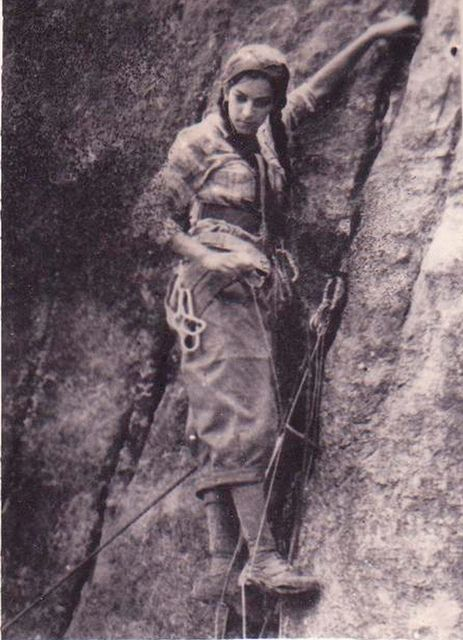
\includegraphics{figs/oldSchoolCool}
          \captionof*{figure}{Archana Bhattacharjee (1979)}
    \vspace{1em}
  \end{minipage}


        \vfill 
\end{multicols}
